\chapter{Band Survey and Capture Sessions}
\label{app:a}

% Approved 2 November 2026 (Chapter 4 outline, decision D2). Filled after the
% band survey and the capture sessions; the session table is to be generated
% from the capture metadata by the report step of code/.

\section{Band Survey}
\label{app:survey}

The survey was made at P1, the sitting-room balcony (\cref{sec:m-sessions}), with the procedure of \cref{sec:m-survey}. The night run began at 22:10 WAT on 4 November 2026 (21:10 UTC) and the day run at 07:00 WAT on 5 November 2026 (06:00 UTC), with the antenna left in place between them. In each run the three candidate ranges were swept one after another, each for \qty{10}{\minute} at a gain of \qty{40.2}{\decibel}, giving 60 readings per frequency bin in bins of about \qty{21}{\kilo\hertz}. The noise floor of each range was the same in both runs to within \qty{0.1}{\decibel}. The cell searches followed each run, between 22:48 and 23:05 and between 07:32 and 07:49 WAT, each from \qty{0.5}{\mega\hertz} below to \qty{0.5}{\mega\hertz} above the plateau's centre, at the same gain and with two tries at each frequency. \Cref{fig:app-survey} shows the mean power in each range, \cref{tab:app-survey} the plateaus found and the result of the cell search on each, and \cref{tab:app-quiet} the quiet stretches that could hold the idle window.

\begin{figure}[tbp]
  \centering
  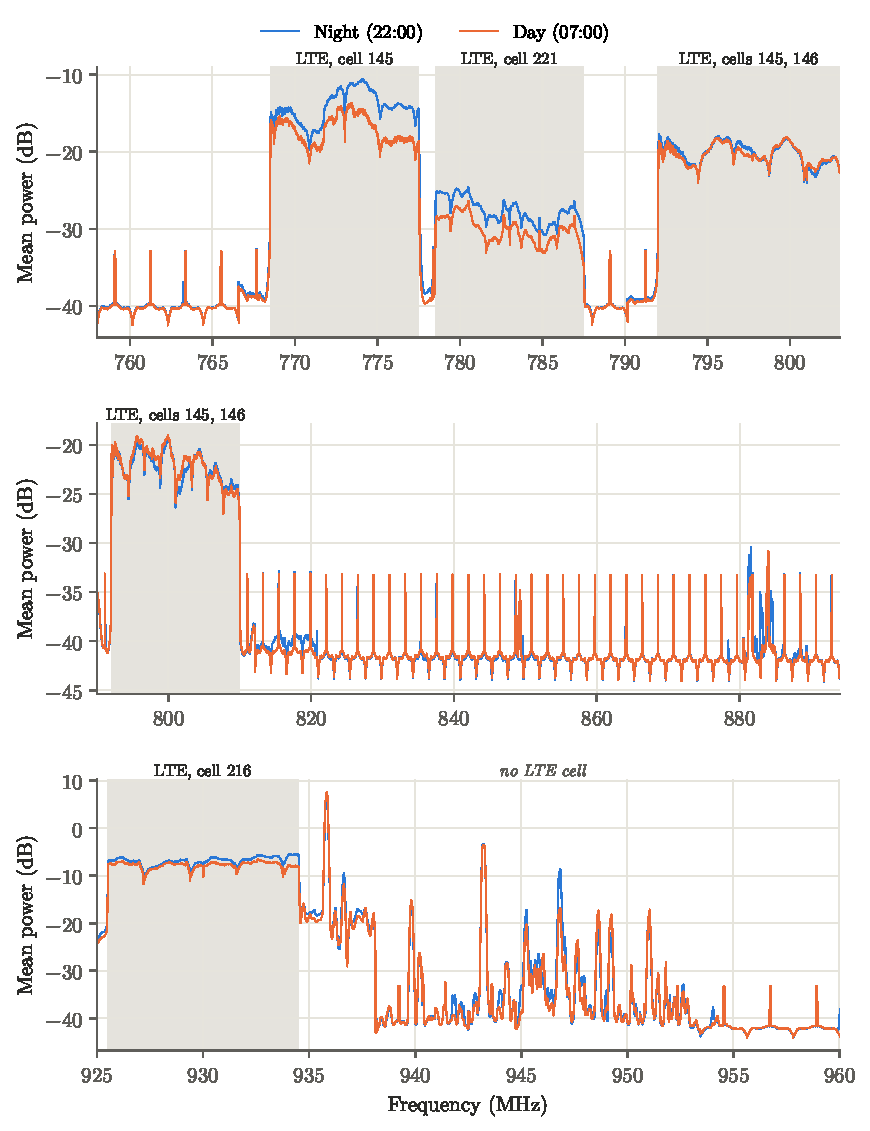
\includegraphics[width=\textwidth]{figA-survey}
  \caption[Band survey at P1]{Band survey at P1 by night and by day: mean power over the 60 readings of each candidate range, on the receiver's uncalibrated scale. Shaded: carriers confirmed by the cell search, drawn over their occupied width (number of resource blocks $\times$ \qty{0.18}{\mega\hertz}). The narrow spikes evenly spaced about \qty{2.2}{\mega\hertz} apart are produced by the receiver at the centre of each tuning step and are not signals.}
  \label{fig:app-survey}
\end{figure}

\begin{table}[tbp]
  \centering
  \small
  \caption[Band survey: plateaus and cell searches]{Band survey at P1: plateaus found in each candidate range and the result of the cell search on each, by night (N, 4 November 2026) and by day (D, 5 November 2026). Frequencies and widths in \unit{\mega\hertz}, from the night run; level in \unit{\decibel}: median mean power of the plateau above the noise floor of its range. The received power is as reported by the cell-search program, on its own relative scale.}
  \label{tab:app-survey}
  \begin{tabularx}{\textwidth}{@{} l l r l >{\raggedright\arraybackslash}X @{}}
    \toprule
    Range & Plateau & Width & Level N / D & Cell search (N and D) \\
    \midrule
    758--803 & 768.4--777.7 & 9.23 & 26.1 / 22.9 & LTE, FDD, cell 145, 50 resource blocks (\qty{10}{\mega\hertz}), centre \qty{773}{\mega\hertz}; \qty{-10.1}{} / \qty{-9.5}{\decibel} \\
     & 778.3--787.5 & 9.18 & 12.7 / 10.3 & LTE, FDD, cell 221, 50 resource blocks (\qty{10}{\mega\hertz}), centre \qty{783}{\mega\hertz}; \qty{-25.8}{} / \qty{-26.2}{\decibel} \\
     & 792.0--803.0 & 11.07 & 20.3 / 20.0 & Cut off at the end of the range; searched in the next range \\
    790--894 & 792.0--810.1 & 18.10 & 20.8 / 21.3 & LTE, FDD, cells 145 and 146, 100 resource blocks (\qty{20}{\mega\hertz}), centre \qty{801}{\mega\hertz}; \qty{-19.3}{} and \qty{-20.1}{} / \qty{-20.8}{} and \qty{-22.5}{\decibel} \\
    925--960 & 925.0--938.2 & 13.18 & 35.1 / 34.2 & A flat part, 925.5--934.5~MHz, followed by narrow peaks; searched at the centre of the flat part: LTE, FDD, cell 216, 50 resource blocks (\qty{10}{\mega\hertz}), centre \qty{930}{\mega\hertz}; \qty{-8.0}{} / \qty{-16.5}{\decibel} \\
     & 944.9--947.3 & 2.36 & 11.7 / 11.1 & No LTE cell found in either run (a cluster of narrow peaks, \qty{1.17}{\mega\hertz} wide by day) \\
    \bottomrule
  \end{tabularx}
\end{table}

Four LTE carriers were confirmed in both runs, with the same cell identities, and all with a channel bandwidth of at least \qty{10}{\mega\hertz}, so that C\textsubscript{offset} captures are possible on any of them (\cref{sec:m-classes}). Their levels changed by at most \qty{3.2}{\decibel} between night and day. Two cells, 145 and 146, were received on the same carrier at \qty{801}{\mega\hertz}; cell identity 145 was also found on the carrier at \qty{773}{\mega\hertz}. The crystal correction factors reported by the ten successful cell searches lay between 0.99999959 and 1.00000023, a receiver frequency error between \qty{-0.41}{ppm} and \qty{+0.23}{ppm}, within the \qty{1}{ppm} tolerance of the reference oscillator; this supports capturing without frequency correction (\cref{sec:m-capture}). Between 812 and \qty{821}{\mega\hertz} a weak signal was present by night but not by day, so that stretch is quiet only by day (\cref{tab:app-quiet}).

\begin{table}[tbp]
  \centering
  \small
  \caption[Band survey: quiet stretches]{Band survey at P1: quiet stretches at least \qty{1.92}{\mega\hertz} wide in which an idle window could be placed (\cref{sec:m-survey}), by night (N) and by day (D), the centre of the window suggested within each, and the largest mean and maximum power above the noise floor within that window.}
  \label{tab:app-quiet}
  \begin{tabular}{@{} l c l r r r @{}}
    \toprule
    Range (\unit{\mega\hertz}) & Run & Stretch (\unit{\mega\hertz}) & Centre (\unit{\mega\hertz}) & Mean (\unit{\decibel}) & Max.\ (\unit{\decibel}) \\
    \midrule
    758--803 & N & 758.0--763.2 & 760.6 & 0.8 & 1.5 \\
     & N & 763.2--766.6 & 764.9 & 0.8 & 1.4 \\
     & N & 787.5--791.9 & 789.7 & 1.7 & 2.7 \\
     & D & 758.0--766.6 & 762.3 & 0.8 & 1.4 \\
     & D & 787.5--791.9 & 789.7 & 1.4 & 3.1 \\
    790--894 & N & 820.8--834.3 & 827.6 & 1.8 & 2.7 \\
     & N & 834.4--849.6 & 842.0 & 1.9 & 3.4 \\
     & N & 849.6--864.0 & 856.8 & 1.8 & 2.5 \\
     & N & 864.0--878.4 & 871.2 & 1.7 & 2.4 \\
     & N & 889.5--894.0 & 891.8 & 1.6 & 2.5 \\
     & D & 812.2--849.0 & 830.6 & 1.9 & 3.3 \\
     & D & 849.4--864.0 & 856.7 & 1.8 & 3.0 \\
     & D & 864.0--880.5 & 872.3 & 1.6 & 2.6 \\
     & D & 885.2--894.0 & 889.6 & 1.9 & 5.3 \\
    925--960 & N & 954.3--960.0 & 957.1 & 0.6 & 1.1 \\
     & D & 952.9--960.0 & 956.5 & 0.7 & 1.3 \\
    \bottomrule
  \end{tabular}
\end{table}

\emph{Choice of band, carrier and idle window.} The band studied is \TargetBand, and the carrier used for the active captures is the \qty{10}{\mega\hertz} carrier centred at \qty{773}{\mega\hertz} (cell identity 145); the choice was confirmed by the author on 5 November 2026. This carrier was strong and steady, \qtyrange{22.9}{26.1}{\decibel} above the noise floor in the two runs; a single cell was received on it; and its bandwidth allows C\textsubscript{offset} captures. Most importantly, the stretch from 758.0 to \qty{766.6}{\mega\hertz} beside it was quiet in both runs, so that the idle window could be placed in the same band, close to the carrier and away from any narrow or intermittent signal. The idle window is centred at \qty{765.37}{\mega\hertz} (\qtyrange{764.41}{766.33}{\mega\hertz}), the window suggested nearest the carrier in both runs: within it, the mean power stayed within \qty{0.8}{\decibel} and the maximum within \qty{1.6}{\decibel} of the noise floor, and it lies about \qty{2.2}{\mega\hertz} below the band occupied by the carrier. The C\textsubscript{offset} window is placed above the carrier's centre, at \qty{775.52}{\mega\hertz}, in every session. The other confirmed carriers were less suitable. The carrier at \qty{783}{\mega\hertz} was \qtyrange{12.6}{13.4}{\decibel} weaker; the one at \qty{801}{\mega\hertz} carried two cells, and the stretch beside it, from 812 to \qty{821}{\mega\hertz}, was quiet only by day; and the one at \qty{930}{\mega\hertz} was strong enough to risk clipping, with narrow peaks between it and its nearest quiet stretch, about \qty{27}{\mega\hertz} away.

\section{Choice of the Gains}
\label{app:gains}

The gains $g_1$ and $g_2$ were chosen with trial captures on 5 November 2026, between 07:57 and 08:02 WAT, at P1 with the antenna as in the survey (\cref{sec:m-capture}). The captures were made with the study's capture program under the session identifier \texttt{trial}, and were then moved out of the data folder, to \texttt{data/trials/2026-11-05\_gain\_trials/}, so that they are never used as study data. The commands were, with \texttt{G} the tuner gain step of each capture:
\begin{lstlisting}[language=bash]
# carrier: 2 s captures at G = 40.2, 38.6, 37.2, 36.4, 33.8, 32.8, 29.7, 28.0, 25.4,
# 22.9 and 20.7 dB, then once more at 37.2 dB
uv run python -m occupancy capture --session trial --position P1 --class C_centre --gain-role g1 --gain G --freq 773M --duration 2 --notes "gain trial"
# idle window: 2 s captures at G = 29.7 and 19.7 dB
uv run python -m occupancy capture --session trial --position P1 --class B --gain-role g1 --gain G --freq 765.37M --duration 2 --notes "gain trial"
# carrier: one full-length (30 s) capture at 29.7 dB
uv run python -m occupancy capture --session trial --position P1 --class C_centre --gain-role g1 --gain 29.7 --freq 773M --duration 30 --notes "gain trial"
# idle window: 2 s captures at G = 22.9, 25.4, 29.7, 33.8, 36.4, 38.6, 40.2, 42.1, 44.5,
# 48.0 and 49.6 dB
uv run python -m occupancy capture --session trial --position P1 --class B --gain-role g1 --gain G --freq 765.37M --duration 2 --notes "gain trial: idle level vs gain"
# summary of all trial captures (Tables A.3 and A.4, Figure A.2)
uv run python -m occupancy trials data/trials/2026-11-05_gain_trials --out ../results/gain_trials_2026-11-05.csv
\end{lstlisting}
The capture program records the fraction of clipped samples and the mean power of each capture; the summary adds the standard deviation of the samples in converter steps and, for captures of at least \qty{10}{\second}, the mean power in blocks of \qty{0.5}{\second}. \Cref{tab:app-gain-carrier,tab:app-gain-idle} list every trial, and \cref{fig:app-gains} plots them.

\begin{table}[tbp]
  \centering
  \small
  \caption[Gain trials: captures centred on the carrier]{Gain trials, 5 November 2026: captures centred on the carrier (\qty{773}{\mega\hertz}), \qty{2}{\second} long unless stated. Time in WAT; gain and mean power in \unit{\decibel}; clipping: percentage of clipped samples (flagged above \pct{0.1}).}
  \label{tab:app-gain-carrier}
  \begin{tabularx}{\textwidth}{@{} l r r r >{\raggedright\arraybackslash}X @{}}
    \toprule
    Time & Gain & Clipping (\%) & Mean power & Note \\
    \midrule
    07:57:15 & \num{40.2} & \num{0.4365} & \num{-9.62} &  \\
    07:57:25 & \num{38.6} & \num{0.1725} & \num{-9.93} &  \\
    07:57:29 & \num{37.2} & \num{0.0812} & \num{-10.58} &  \\
    07:57:33 & \num{36.4} & \num{0.0276} & \num{-10.80} &  \\
    07:57:37 & \num{33.8} & \num{0.0012} & \num{-14.52} &  \\
    07:57:41 & \num{32.8} & \num{0.00003} & \num{-16.02} &  \\
    07:57:45 & \num{29.7} & 0 & \num{-19.34} &  \\
    07:57:49 & \num{28.0} & 0 & \num{-20.13} &  \\
    07:57:53 & \num{25.4} & 0 & \num{-22.13} &  \\
    07:57:57 & \num{22.9} & 0 & \num{-23.28} &  \\
    07:58:01 & \num{20.7} & 0 & \num{-27.53} &  \\
    07:58:11 & \num{37.2} & \num{2.6958} & \num{-3.93} & Repeat during a traffic peak \\
    07:59:25 & \num{29.7} & 0 & \num{-21.48} & \qty{30}{\second} capture; \qty{0.5}{\second} block power \numrange{-23.0}{-18.0}~dB \\
    \bottomrule
  \end{tabularx}
\end{table}

\begin{table}[tbp]
  \centering
  \small
  \caption[Gain trials: idle captures]{Gain trials, 5 November 2026: \qty{2}{\second} captures of the idle window (\qty{765.37}{\mega\hertz}), by gain. Time in WAT; gain and mean power in \unit{\decibel}; standard deviation of the in-phase and quadrature samples in converter steps. No sample was clipped.}
  \label{tab:app-gain-idle}
  \begin{tabular}{@{} l r r r @{}}
    \toprule
    Time & Gain & Mean power & Standard deviation \\
    \midrule
    07:59:21 & \num{19.7} & \num{-42.35} & \num{0.68} \\
    08:00:54 & \num{22.9} & \num{-41.86} & \num{0.72} \\
    08:00:58 & \num{25.4} & \num{-41.40} & \num{0.76} \\
    07:59:17 & \num{29.7} & \num{-40.34} & \num{0.86} \\
    08:01:02 & \num{29.7} & \num{-40.38} & \num{0.86} \\
    08:01:06 & \num{33.8} & \num{-38.81} & \num{1.03} \\
    08:01:10 & \num{36.4} & \num{-37.85} & \num{1.15} \\
    08:01:14 & \num{38.6} & \num{-35.95} & \num{1.43} \\
    08:01:18 & \num{40.2} & \num{-34.83} & \num{1.63} \\
    08:01:22 & \num{42.1} & \num{-34.09} & \num{1.78} \\
    08:01:26 & \num{44.5} & \num{-32.83} & \num{2.06} \\
    08:01:30 & \num{48.0} & \num{-31.07} & \num{2.52} \\
    08:01:34 & \num{49.6} & \num{-32.08} & \num{2.24} \\
    \bottomrule
  \end{tabular}
\end{table}

\begin{figure}[tbp]
  \centering
  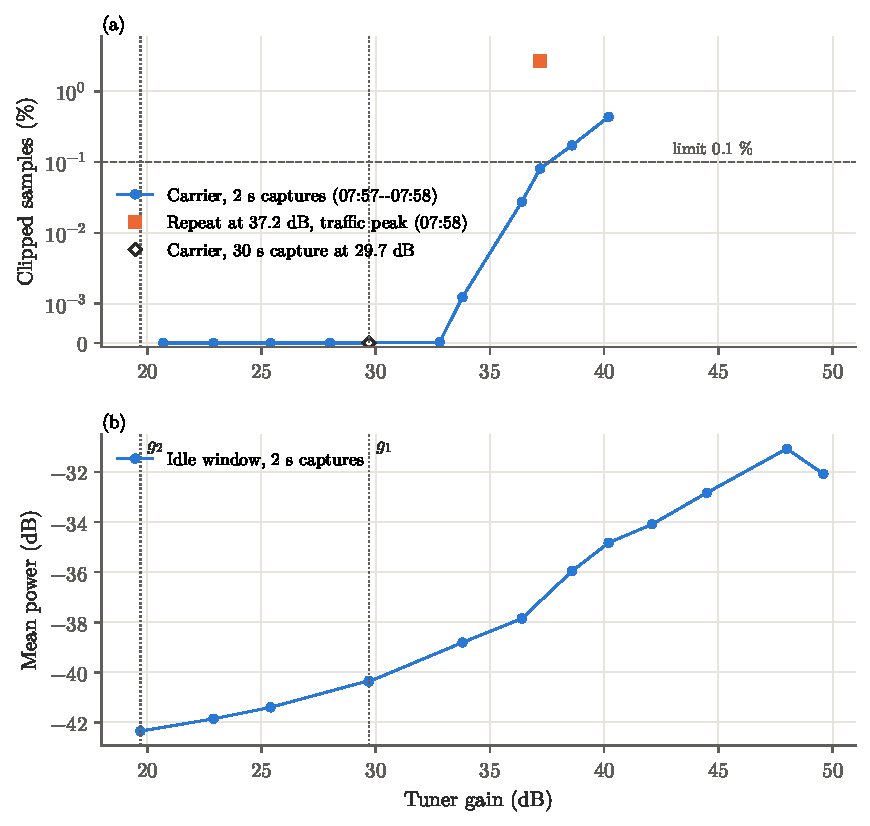
\includegraphics[width=\textwidth]{figA-gains}
  \caption[Gain trials]{Gain trials at P1, 5 November 2026. (a) Clipped samples in captures centred on the carrier, against the tuner gain, on a scale that is linear near zero and logarithmic above \pct{0.001}; the dashed line is the \pct{0.1} limit. (b) Mean power of captures of the idle window against the gain. Dotted lines: the chosen gains $g_1$ and $g_2$. Data of \cref{tab:app-gain-carrier,tab:app-gain-idle}.}
  \label{fig:app-gains}
\end{figure}

\emph{Choice of $g_1$.} Applied to the first series of carrier captures alone, the clipping limit would have given $g_1 = \qty{37.2}{\decibel}$, where \pct{0.081} of the samples clipped. A repeat at that gain about \qty{40}{\second} later, however, clipped \pct{2.70} of the samples: the carrier's mean power was \qty{6.7}{\decibel} higher (\qty{-3.93}{} against \qty{-10.58}{\decibel}), most probably because the power of a downlink carrier rises and falls with its traffic, whereas only its reference signals are always transmitted (\cref{sec:lte-sync}). A gain that respects the limit only when traffic is quiet would make clipped captures, which would have to be retaken, frequent at busy times. Retaking them until traffic is quiet would bias the data towards low traffic, so $g_1$ was instead chosen with a margin for such peaks: $g_1 = \qty{29.7}{\decibel}$, \qty{7.5}{\decibel} below \qty{37.2}{\decibel}. A traffic peak of the size observed brings the carrier at this gain to about the level it had at \qty{36.4}{\decibel} in quiet traffic, where \pct{0.028} of the samples clipped. A full-length capture at \qty{29.7}{\decibel}, during which the mean power in \qty{0.5}{\second} blocks varied over \qty{5.0}{\decibel}, had no clipped samples. The second gain is the tuner step \qty{10}{\decibel} lower, $g_2 = \qty{19.7}{\decibel}$, as agreed before the trials. Two alternatives were considered and set aside by the author: changing to the weaker carrier at \qty{783}{\mega\hertz}, which would have allowed a higher gain but would have reopened the choice of carrier and idle window, and a higher $g_1$ with clipped captures retaken, which would have biased the data as described above. The gains were confirmed by the author on 5 November 2026.

\emph{Consequence for the idle data.} Below about \qty{30}{\decibel} the idle level changed little with the gain: from \qty{-41.86}{\decibel} at \qty{22.9}{\decibel} to \qty{-40.38}{\decibel} at \qty{29.7}{\decibel}, \qty{1.5}{\decibel} for \qty{6.8}{\decibel} of gain. Above it, the level rose by roughly half a decibel per decibel of gain (\cref{fig:app-gains}). At these gains the idle level is therefore set mainly by the receiver's own noise rather than by what the antenna receives; at $g_1$ the idle samples had a standard deviation of only \num{0.86} converter steps. Lowering the gain from $g_1$ to $g_2$ lowered the idle level by \qty{2.0}{\decibel} (\qty{-40.34}{} to \qty{-42.35}{\decibel}), while the carrier fell by \qty{8.2}{\decibel} between \qty{29.7}{} and \qty{20.7}{\decibel}. Two expectations follow, and both are checked in every session: the captures with the antenna terminated (Class~A) and connected (Class~B) should differ little, and the gain-change test of H2 shifts the idle level by about \qty{2}{\decibel} rather than \qty{10}{\decibel} (\cref{sec:m-robustness}).

\section{Capture Sessions}
\label{app:sessions}

\TBC{One row per session: identifier, date and start time (UTC), position, gain settings $g_1$ and $g_2$, captures made, clipping flags and notes (\cref{sec:m-sessions}).}
